% !TeX root=../main.tex

\chapter{مقدمه و بیان مسئله}
% دستور زیر باعث عدم‌نمایش شماره صفحه در اولین صفحهٔ این فصل می‌شود.
%\thispagestyle{empty}

% ------------ Section 2
\section{مقدمه}
در یک دهه اخیر محبوبیت رمزارز‌ها در میان مردم به شدت افزایش داشته است. رمزارزها توکن هایی تعویض پذیر هستند به این معنی که تفاوتی میان دو توکن یک
\gls{CryptoCurrency}
وجود ندارد، مانند پول فیزیکی که ارزش یک هزار تومانی با یک هزار تومانی دیگر تفاوتی ندارد.
اما در دنیای واقعی تنها مالکیت پول وجود ندارد، بلکه یک فرد میتواند خودرو، خانه، بلیت هواپیمای و دیگر دارایی‌هایی داشته باشد که یکتا هستند و با هیچ دارایی دیگری دقیقا یکسان نیستند. مثلا یک بلیت هواپیما برای یک تاریخ و ساعت خاص برای یک شماره پرواز خاص از یک مبدا مشخص به یک مقصد مشخص است و شماره صندلی یکتایی نیز دارد. پس هیچ دو بلیت هواپیمایی دقیقا یکسان نیستند، بر خلاف دو بیتکوین که کاملا یکسان هستند، ارزش برابری دارند، و تعویض پذیر هستند.
کاربردهای
\glspl{Non-fungible token}
بیشمار است و در حال حاضر فقط قسمت اندکی از کاربردهایی که میتوانند داشته باشند را پاسخ گفته‌اند. در این پروژه پلتفرمی می‌سازیم که ساخت و انتقال
\gls{Non-fungible token}
را برای عموم در دسترس‌تر و آسان‌تر کند. همچنین یکی از اهدف انجام این پروژه آشنایی با تکنولوژی‌ها، استاندارد‌ها و فرایند‌های این توکن‌هاست.

% ------------ Section 2
\section{شرح مسئله و روش انجام آن}
کلیه فایل‌های لازم برای حروف‌چینی با کلاس فوق، داخل پوشه‌ای به نام
\lr{tehran-thesis}
قرار داده شده است. توجه داشته باشید که برای استفاده از این کلاس باید فونت‌های
\lr{IRLotusICEE}
و
\lr{IRTitr}
را داشته باشید (که همراه با این کلاس هست و نیاز به نصب نیست).
قلم‌های
\lr{IRLotusICEE}
مستخرج از قلم‌های استاندارد
\lr{IRLotus}
شورای عالی اطلاع‌رسانی%
\footnote{
قلم‌های استاندارد
\lr{IRFonts}
از شورای عالی اطلاع‌رسانی، منطبق بر آخرین نسخه استاندارد یونیکد، استاندارد ملی ۶۲۱۹ و استاندارد
\lr{Adobe Glyph Naming}
هستند.
}
هستند که توسط دکتر بابایی‌زاده اصلاحاتی روی آنها صورت پذیرفته است: تبدیل صفر توپر به صفر توخالی (جهت تمایز بیشتر با نقطه) و اضافه شدن
\textit{\textbf{حالت توپر و ایرانیک توأم}}،
که این موارد در قلم‌های شورای عالی اطلاع‌رسانی وجود ندارد.

\subsection{این همه فایل؟!}
\label{muchFiles}
از آنجایی که یک پایان‌نامه یا رساله، یک نوشته بلند محسوب می‌شود، لذا اگر همه تنظیمات و مطالب پایان‌نامه را داخل یک فایل قرار بدهیم، باعث شلوغی و سردرگمی می‌شود. به همین خاطر، قسمت‌های مختلف پایان‌نامه یا رساله  داخل فایل‌های جداگانه قرار گرفته است. مثلاً تنظیمات پایه‌ای کلاس داخل فایل
\lr{tehran-thesis.cls}، 
قسمت مشخصات فارسی پایان‌نامه داخل 
\lr{faTitle.tex}،
مطالب فصل اول داخل 
\lr{chapter1.tex}
و تنظیمات قابل تغییر توسط کاربر داخل 
\lr{commands.tex}،
قرار داده شده است.
\textbf{
	فایل اصلی این مجموعه، فایل
	\lr{main.tex}
	می‌باشد.
}
% یعنی بعد از تغییر فایل‌های دیگر، برای دیدن نتیجه تغییرات، باید این فایل را اجرا کرد. بقیه فایل‌ها به این فایل، کمک می‌کنند تا بتوانیم خروجی کار را ببینیم.
اگر به فایل 
\lr{main.tex}
دقت کنید، متوجه می‌شوید که قسمت‌های مختلف پایان‌نامه، توسط دستورهایی مانند 
\lr{input}
و
\lr{include}
به فایل اصلی، یعنی 
\lr{main.tex}
معرفی شده‌اند.
با توجه به ساختار محتوایی دستورالعمل، در فایل
\lr{main.tex}
فرض شده که پایان‌نامه یا رساله شما، از ۵ فصل و تعدادی پیوست تشکیل شده است. با اینحال، شما می‌توانید به راحتی فصل‌ها و پیوست‌ها را با صلاحدید اساتید راهنما، کم و زیاد کنید. این کار، بسیار ساده است. فرض کنید بخواهید یک فصل دیگر هم به پایان‌نامه اضافه کنید. برای این کار، کافی است یک فایل با نام دلخواه مثلاً 
\lr{chapter6}
و با پسوند 
\lr{.tex}
بسازید و آن را داخل پوشه 
\lr{tehran-thesis}
قرار دهید و سپس این فایل را با دستور 
\verb!\include{chapter6}!
داخل فایل
\lr{main.tex}
 فراخوانی کنید.

\subsection{از کجا شروع کنم؟}
قبل از هر چیز، باید یک توزیع تِک مناسب مانند تک‌لایو
\lr{(TeXLive)}
را روی سیستم خود نصب کنید. تک‌لایو  را می‌توانید از 
 \href{http://www.tug.org/texlive}{سایت رسمی آن}%
\LTRfootnote{\lr{\url{http://www.tug.org/texlive}}}
 دانلود کنید یا مستقیماً از مخازن توزیع لینوکس خود بگیرید (مثلاً در اوبونتو با دستور
\LRE{\verb!sudo apt install texlive-full!}).
برای نصب تک‌لایو و اجرای اسناد زی‌پرشین می‌توانید از
\href{http://parsilatex.com/site/shop/}{دی‌وی‌دی مجموعه پارسی‌لاتک}%
\LTRfootnote{\lr{\url{http://parsilatex.com/site/shop/}}}
و فایل راهنمای موجود در آن هم کمک بگیرید.

برای تایپ و پردازش اسناد لاتک باید از یک ویرایشگر مناسب استفاده کنید. ویرایشگرهای
\lr{TeXWroks},
\lr{TeXstudio},
\lr{Texmaker}
و
\lr{BiDiTeXmaker}
بدین منظور تولید شده‌اند. می‌توان ویرایش‌گر 
 \href{https://bitbucket.org/srazi/biditexmaker3}{\lr{BiDiTeXmaker}}%
 \LTRfootnote{\lr{\url{https://bitbucket.org/srazi/biditexmaker3}}}
را که بویژه برای کار با زی‌پرشین و مطالب دوجهته بهبود یافته است، بهینه‌ترین ویرایشگر لاتک برای کار با اسناد فارسی عنوان کرد.
 
حال اگر نوشتن \پ اولین تجربه شما از کار با لاتک است، توصیه می‌شود که یک‌بار به صورت اجمالی، کتاب «%
\href{http://www.tug.ctan.org/tex-archive/info/lshort/persian/lshort.pdf}{مقدمه‌ای نه چندان کوتاه بر
\lr{\LaTeXe}}%
\LTRfootnote{\lr{\url{http://www.tug.ctan.org/tex-archive/info/lshort/persian/lshort.pdf}\hfill}}»
ترجمه دکتر مهدی امیدعلی را مطالعه کنید. این کتاب، کتاب بسیار کاملی است که خیلی از نیازهای شما در ارتباط با حروف‌چینی را برطرف می‌کند.
اگر تک لایو کامل را داشته باشید، این کتاب را هم دارید. کافیست در خط فرمان دستور زیر را بزنید:
\begin{latin}
	\texttt{texdoc lshort-persian}
\end{latin}
اگر عجله دارید، برخی دستورات پایه‌ای مورد نیاز در پیوست \ref{app:latexIntro} بیان شده‌اند.
 
بعد از موارد گفته شده، فایل 
\lr{main.tex}
و
\lr{faTitle.tex}
را باز کنید و مشخصات پایان‌نامه خود مثل نام، نام خانوادگی، عنوان پایان‌نامه و ... را جایگزین مشخصات موجود در فایل
\lr{faTitle.tex}
 کنید. نیازی نیست نگران چینش این مشخصات در فایل پی‌دی‌اف خروجی باشید، زیرا کلاس 
\lr{tehran-thesis}
همه این کارها را بطور خودکار برای شما انجام می‌دهد. در ضمن، موقع تغییر دادن دستورهای داخل فایل
\lr{faTitle.tex}
 کاملاً دقت کنید؛ این دستورها، خیلی حساس هستند و ممکن است با یک تغییر کوچک، موقع اجرا، خطا بگیرید. برای دیدن خروجی کار، فایل 
\lr{faTitle.tex}
 را 
\lr{Save}
(نه 
\lr{Save As})
کنید و بعد به فایل 
\lr{main.tex}
برگشته و آن را اجرا کنید%
\footnote{
	البته فایلهای این مجموعه به گونه‌ای هستند که در
	\lr{TeXWorks} یا
	\lr{TeXstudio}
	بدون بازگشت به فایل اصلی، می‌توانید سند خود را اجرا کنید.
}.
 حال اگر می‌خواهید مشخصات انگلیسی \پ را هم عوض کنید، فایل 
\lr{enTitle.tex}
را باز کنید و مشخصات داخلش را تغییر دهید.
%\RTLfootnote{
%برای نوشتن پروژه کارشناسی، نیازی به وارد کردن مشخصات انگلیسی پروژه نیست. بنابراین، این مشخصات بطور خودکار، نادیده گرفته می‌شود.
%}
در اینجا هم برای دیدن خروجی باید این فایل را ذخیره کرده، بعد به فایل 
\lr{main.tex}
برگشته و آن را اجرا کرد.

برای راحتی بیشتر، کلاس 
\lr{tehran-thesis.cls}
طوری طراحی شده است که کافی است فقط  یک‌بار مشخصات \پ را (در فایل‌های
\lr{faTitle.tex}
و
\lr{enTitle.tex})
وارد کنید و هر جای دیگر که این مشخصات لازم باشند، به طور خودکار درج می‌شوند. با این حال، اگر مایل بودید، می‌توانید تنظیمات موجود را تغییر دهید؛ گرچه، در صورتیکه کاربر مبتدی هستید و یا با ساختار فایل‌های  
\lr{cls}
 آشنایی ندارید، بهتر است به فایل 
\lr{tehran-thesis.cls}
دست نزنید.

نکته دیگری که باید به آن توجه کنید این است که در قالب آماده شده، سه گزینه به نام‌های
\lr{bsc}،
\lr{msc}
و
\lr{phd}
برای نوشتن پروژه، پایان‌نامه و رساله، در نظر گرفته شده است. بنابراین اگر قصد تایپ پروژهٔ کارشناسی، پایان‌نامهٔ کارشناسی ارشد یا رسالهٔ دکتری را دارید، به ترتیب باید از گزینه‌های
\lr{bsc}،
\lr{msc}
و
\lr{phd}
در فایل 
\lr{main.tex}
استفاده کنید. با انتخاب هر کدام از این گزینه‌ها، تنظیمات مربوط به آنها به طور خودکار، اعمال می‌شود.


\subsection[مطالب پایان‌نامه را چطور بنویسم؟]
{مطالب \پ را چطور بنویسم؟}
\subsubsection{نوشتن فصل‌ها}
همان‌طور که در بخش \ref{muchFiles} گفته شد برای جلوگیری از شلوغی، قسمت‌های مختلف \پ از جمله فصل‌ها، در فایل‌های جداگانه‌ای قرار داده شده‌اند. 
مثلاً اگر می‌خواهید مطالب فصل ۱ را تایپ کنید، باید فایل‌های 
\lr{main.tex}
و
\lr{chapter1.tex}
را باز کرده و مطالب خود را جایگزین محتویات داخل 
\lr{chapter1.tex}
نمایید. دقت شود که در ابتدای برخی فایلها دستوراتی نوشته شده است و از شما خواسته شده که آن دستورات را حذف نکنید.

%توجه کنید که همان‌طور که قبلاً هم گفته شد، تنها فایل قابل اجرا، 
%\lr{main.tex}
%است. لذا برای دیدن حاصل (خروجی) فایل خود، باید  
%\lr{chapter1.tex}
%را ذخیره کرده و سپس فایل 
%\lr{main.tex}
%را اجرا کنید.

نکته بسیار مهمی که در اینجا باید گفته شود این است که سیستم \lr{\TeX}، محتویات یک فایل تِک را به ترتیب پردازش می‌کند.  بنابراین، اگر مثلاً  دو فصل اول خود را نوشته و خروجی آنها را دیده‌اید و مشغول تایپ مطالب فصل ۳ هستید، بهتر است
که دو دستور 
\verb!% !TeX root=../main.tex

\chapter{مقدمه و بیان مسئله}
% دستور زیر باعث عدم‌نمایش شماره صفحه در اولین صفحهٔ این فصل می‌شود.
%\thispagestyle{empty}

% ------------ Section 1.1 ------------
\section{مقدمه}
در یک دهه اخیر محبوبیت رمزارز‌ها در میان مردم به شدت افزایش داشته است. رمزارزها توکن هایی تعویض پذیر هستند به این معنی که تفاوتی میان دو توکن یک
\gls{CryptoCurrency}
وجود ندارد، مانند
\gls{Fiat Money}
که ارزش یک هزار تومانی با یک هزار تومانی دیگر تفاوتی ندارد.

اما در دنیای واقعی تنها مالکیت پول نیست که اهمیت دارد، بلکه یک فرد می‌تواند خودرو، خانه، بلیت هواپیما و دیگر دارایی‌هایی داشته باشد که یکتا هستند و با هیچ دارایی دیگری دقیقا یکسان نیستند. مثلا یک بلیت هواپیما برای تاریخ و ساعتی خاص برای شماره پروازی خاص از یک مبدا مشخص به یک مقصد مشخص است و شماره صندلی یکتایی نیز دارد. پس هیچ دو بلیت هواپیمایی دقیقا یکسان نیستند، بر خلاف دو بیتکوین که کاملا یکسان هستند، ارزش برابری دارند، و تعویض پذیر هستند.

کاربردهای توکن‌های تعویض ناپذیر بیشمار است و در حال حاضر فقط قسمت اندکی از کاربردهایی که می‌توانند داشته باشند را پاسخ گفته‌اند. در این پروژه یک
\gls{Platform}
می‌سازیم که ساخت و انتقال توکن‌های تعویض ناپذیر را برای عموم در دسترس‌تر و آسان‌تر می‌کند. همچنین یکی از اهداف انجام این پروژه آشنایی با تکنولوژی‌ها، استاندارد‌ها و فرایند‌های توسعه این توکن‌هاست.


% ------------ Section 1.2
\section{شرح مسئله و روش انجام آن}
پروژه تعریف شده توسعه یک پلتفرم برای
\gls{Mint}
و انتقال توکن‌های تعویض ناپذیر به آسان‌ترین روش ممکن است، به نحوی که برای هر کسی به راحتی در دسترس باشد. نکته‌ی قابل توجه‌ این است که در مسیر انجام این پروژه با تکنولوژی‌های موجود در این زمینه، فریمورک‌ها، استاندارد‌ها و فرایند تست و دیپلوی آشنا شویم.

برای انجام این مراحل در قدم اول نحوه توسعه اپلیکیشن‌های غیرمتمرکز و برتری‌های نوشتن پروژه به صورت متن‌باز ذکر می‌شود، سپس فریمورک‌ها و ابزار‌هایی که برای ساخت یک اپلیکیشن غیرمتمرکز به توسعه دهنده کمک می‌کنند معرفی می‌شوند و نحوه استفاده از آن‌ها شرح داده می‌شود.

سپس فرایند توسعه آغاز می‌شود، استاندارد‌های موجود برای نوشتن یک قرارداد برای توکن‌های تعویض ناپذیر شرح داده می‌شود و کاپو تا جای ممکن مطابق آن‌ها توسعه می‌یابد. برای قرارداد هوشمند نوشته شده تست می‌نویسیم و آن را روی
\gls{Testnet}
انتشار می‌دهیم.
در گام بعد برای پلتفرم، فرانت‌اند ساده‌ای نوشته می‌شود که با قرارداد هوشمند و همچنین کیف پول دیجیتال کاربر ارتباط برقرار می‌کند و سپس به کمک
\gls{Github Pages}
دیپلوی می‌شود تا در دسترس عموم کاربرها قرار بگیرد.

برای
\gls{Dockerize}
کردن تست‌های
\gls{Smart Contract}
یک
\gls{Docker Image}
\gls{Truffle}
نوشته می‌شود. در قدم بعد هر دو بخش فرانت و قرارداد هوشمند داکرایز می‌شوند و فرایند اجرای تست‌های قرارداد هوشمند و دیپلوی شدن فرانت به صورت خودکار به کمک پایپلاین‌های گیت‌هاب پیاده‌سازی می‌شود.


% ------------ Section 1.3
\section{اهداف کلی تحقیق}
اهداف این تحقیق را می‌توان به دو دسته تقسیم‌بندی نمود.

\subsection{گسترش کاربرد‌های توکن‌های تعویض ناپذیر}
این توکن‌ها در همین مدت کوتاهی که به وجود آمده‌اند کاربردهای فراوانی را پوشش داده‌اند. اما همچنان قسمت بزرگی از این کاربردها صرفا ثبت مالکیت آثار هنری دیجیتال است. درحالی که توکن‌های داده‌ای می‌توانند وسعت بسیار عظیم‌تری از کاربردها را پوشش دهند. از کاربردهای روزانه مانند بلیت سینما و هواپیما، تا مالکیت هر نوع دارایی واقعی یا مجازی.

با توجه به نحوه کار اکثر قراردادهای توکن‌های تعویض ناپذیر، معمولا فقط مالک قرارداد می‌تواند توکن ایجاد کند، یا در قرارداد برای ایجاد توکن شرط‌هایی مانند حداکثر تعداد ممکن گذاشته می‌شود. این موضوع به این معنی است که اگر شخصی بخواهد خودش توکن‌هایی ایجاد کند و به دیگران انتقال دهد احتمالا مجبور است که قراردادهوشمند خودش را بنویسد و دیپلوی کند. این فرآیند نیاز به دانش فنی، آشنایی کامل با این زمینه و پرداخت هزینه‌های دیپلوی قرارداد روی شبکه بلاکچین دارد.

کاپو به هر آدرسی اجازه می‌دهد که به راحت‌ترین حالت ممکن و به هر تعداد که مورد نیاز است توکن تعویض ناپذیر روی این قرارداد ایجاد کند. به این ترتیب استفاده از کاپو برای عموم مردم آسان‌تر، ارزان‌تر و در دسترس‌تر است.

\subsection{یادگیری}
هدف دیگر انجام این پروژه یادگیری است. با توجه به رشد سریع و تازگی استفاده از تکنولوژی‌های بلاکچین و توکن‌های تعویض ناپذیر، با وجود تلاش برای ایجاد منابع یادگیری مناسب همچنان فضاهای خالی، کمبودها و نیازمندی‌هایی وجود دارد که باید پاسخ گفته شوند. در طی انجام این پروژه با ابزارها، کتابخانه‌ها، فریمورک‌ها و استانداردهای نوشتن قراردادهای هوشمند آشنا می‌شویم، می‌آموزیم که هر یک چطور کار میکنند و چگونه می‌توانند به توسعه دهنده کمک کنند.

% ------------ Section 1.4
\section{ساختار پایان‌نامه}
پس از این مقدمه، در فصل ۲ مفاهیم اولیه توسعه اپلیکیشن بر بستر بلاک‌چین، کاربردها، مفاهیم و استاندارد‌ها توضیح داده می‌شود. در فصل ۳ ابزار‌های توسعه قرارداد‌های هوشمند معرفی می‌شوند، مزایا و معایب هر یک بیان می‌شود و نحوه استفاده از آن‌ها توضیح داده می‌شود. در فصل ۴ روند پیاده‌سازی شرح داده می‌شود. بررسی می‌شود که در هر مرحله از پیاده‌سازی چه کارهایی به چه ترتیبی انجام شده است. در فصل پنجم نیز نتایج توضیح داده می‌شوند و جمع‌بندی صورت میگیرد.
!
و
\verb!% !TeX root=../main.tex
\chapter{مفاهیم اولیه و پیش‌زمینه}
% ------------ Section 2.1
\section{دلایل و برتری‌های متن‌باز بودن قرارداد‌های هوشمند}
دلایل زیادی برای متن‌باز نوشتن قراردادهای هوشمند وجود دارد، در ادامه تعدادی از این دلایل توضیح داده می‌شود.

دلیل اول، بلاک‌چین‌ها
\gls{Confidentiality}
ندارند، همه‌ی نود‌های شبکه برای اجرای کد قرارداد هوشمند باید حداقل به
\glspl{bytecode}
قرارداد هوشمند دسترسی داشته باشند و این بایت‌کد‌ها در کاوشگرهای بلاکچین نیز وجود دارند، همچنین
\gls{Decompiler}هایی
وجود دارند که از بایت‌کد‌های قرارداد هوشمند کد سالیدیتی آن را به دست می‌آورند. پس در نتیجه تلاش برای مخفی کردن کدهای قرارداد هوشمند بیهوده خواهد بود.

دلیل دوم، اصلی‌ترین مزیت اپلیکیشن‌های غیرمتمرکز نسبت به اپلیکیشن‌های متمرکز عدم نیاز به اعتماد است، کاربرها می‌توانند کد‌های قرارداد هوشمند را بخوانند و به کد نوشته شده اعتماد کنند،‌در حالی که اگر کد برنامه برای همه کاربران قابل مشاهده نباشد کاربرها باید به سازندگان آن برنامه اعتماد کنند.

دلیل سوم، بارگذاری کردن قرارداد‌های هوشمند معمولا آسان نیست و سرعت تغییرات پایین‌تر از اپلیکیشن‌های متمرکز هست،‌ پس امکان این که با پیدا شدن هر مشکل بتوان به سرعت آن را درست کرد کمتر وجود دارد و مسئله امنیت بسیار اهمیت دارد. متن‌باز نوشتن قرارداد هوشمند باعث می‌شود چشم‌های بیشتری کدهای قرارداد را بخوانند و مشکلات احتمالی سریعتر مشخص و رفع شوند. تعداد زیادی از این پروژه‌ها از همان روز اول قرارداد هوشمند را به صورت متن‌باز توسعه می‌دهند، بعضی نیز ترجیح میدهند که پروژه به مرحله‌ای از توسعه برسد و سپس آن را متن‌باز میکنند.

ر این حوضه سرعت پیشرفت و توسعه به دلیل متن باز بودن به شدت بالاست به نحوی که در طی اجرای این پروژه مرج ریکوئستی روی کتابخانه OpenZeppelin زده شد که در همان روز مرج شد. این موضوع علاوه بر این که نشان‌دهنده سرعت پیشرفت بسیار بالاست، این موضوع را نیز نشان میدهد که در یک جامعه متن‌باز هر توسعه دهنده می‌تواند به پیشرفت جامعه به هر شکلی که می‌تواند کمک کند، اشکالاتی که مشاهده می‌کند را گزارش دهد یا تصحیح کند.

\begin{figure}[ht]
\centerline{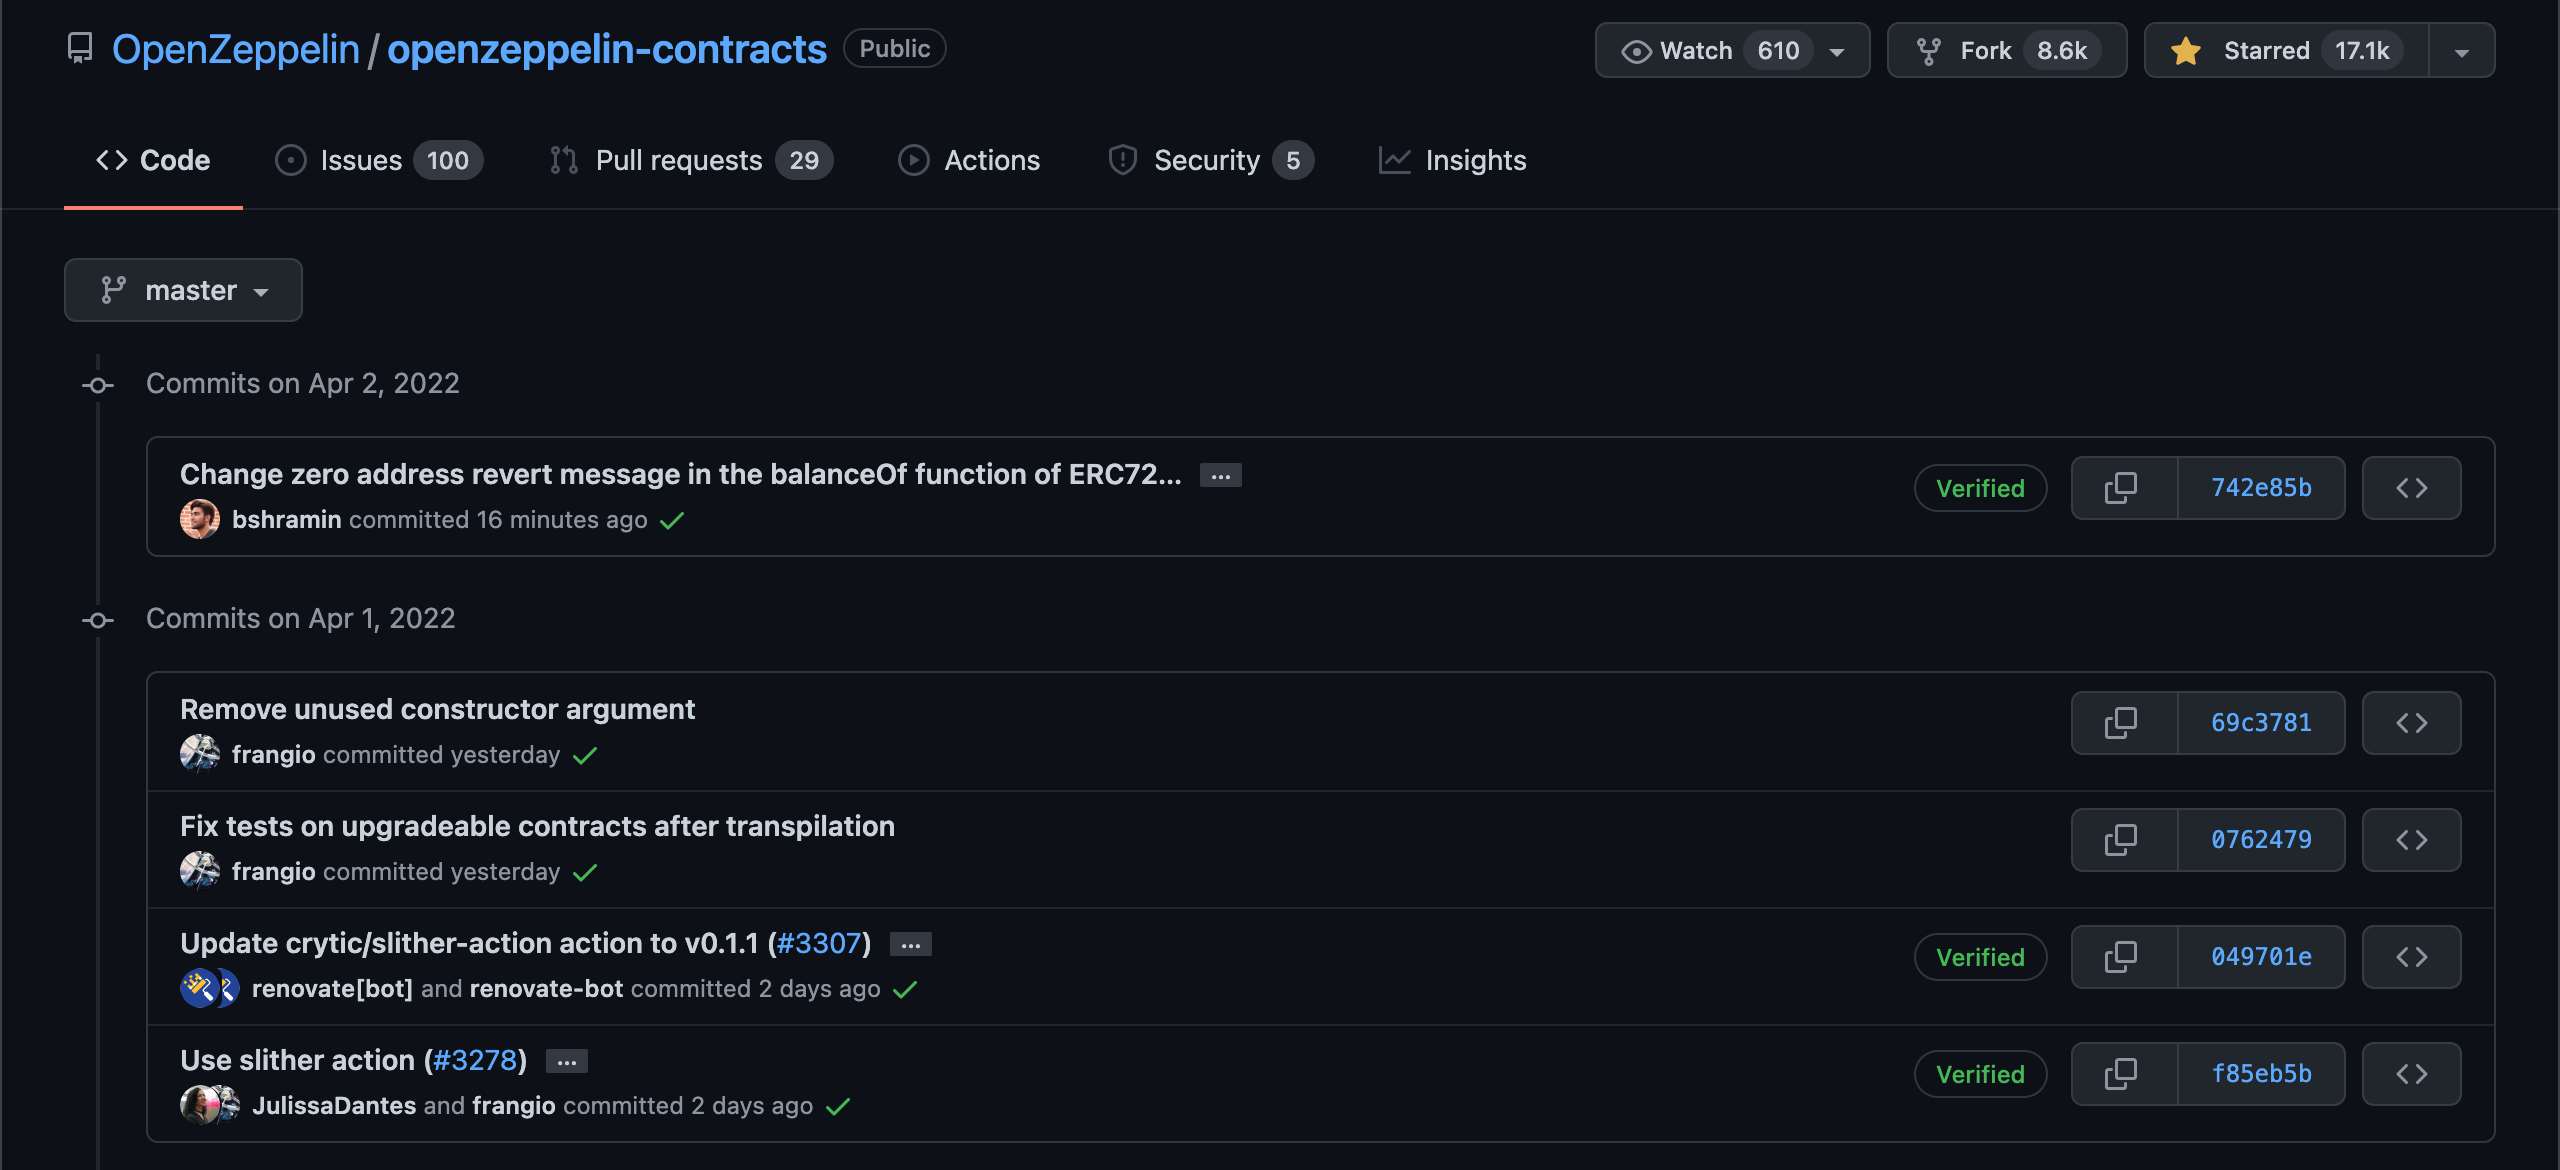
\includegraphics[width=15cm]{OpenZepplinContribution.png}}
\caption{در طی انجام پروژه مرج ریکوئستی روی OpenZeppelin باز شد که در همان روز مرج شد.}
\label{fig:zeppelin-merge-req}
\end{figure}


% ------------ Section 2.2
\section{آشنایی با مفهوم توکن تعویض ناپذیر}
شروع رمزارزها با توکن‌های تعویض پذیر بود، مفهوم تعویض پذیری به این معنی است که یک توکن با توکن دیگر تفاوتی ندارد و با جابه‌جا شدن آن‌ها تغییری ایجاد نمی‌شود. برای مثال یک بیت‌کوین با یک بیت‌کوین دیگر هیچ تفاوتی ندارد.

اما توکن‌های تعویض ناپذیر اینگونه نیستند، هر یک منحصر به فرد است و جابه‌جا کردن آن‌ها با یکدیگر تغییر ایجاد می‌کند،‌ در دنیای واقعی خانه می‌تواند مثال خوبی از یک دارایی تعویض ناپذیر باشد، هیچ دو خانه‌ای دقیقا شبیه به هم، در یک مکان، در طبقه یکسان و دارای پلاک مشترک نیستند.

پس مثلا به عنوان یک کاربرد، شهرداری می‌تواند یک قرارداد هوشمند ایجاد کند و به هر خانه یک توکن NFT اختصاص دهد. به این صورت صاحب خانه به جای سند یک توکن NFT دارد که مشخص می‌کند که دارایی متعلق به اوست، و فروش خانه به راحتی انتقال آن NFT به شخص دیگری است.

از نظر فنی هر توکن به این صورت یکتاست که یک \lr{Token ID} یکتا در قراردادش دارد و هر قرارداد هم دارای یک آدرس یکتا در شبکه بلاکچین است. پس ترکیب Contract Address و \lr{Token ID} باعث می‌شود که هر توکن یکتا باشد.


% ------------ Section 2.3
\section{کاربردها، حال و آینده}
کاربرد NFTها تا به حال در دو دسته خلاصه می‌شود. دسته اول به عنوان صاحب یک اثر دیجیتال، مانند یک تصویر یا یک موسیقی. دسته دوم به عنوان یک جواز یا بلیت برای ورود به جایی یا دریافت چیزی، برای مثال همایشی برگزار می‌شود که فقط دارندگان NFTهای یک قرارداد هوشمند می‌توانند به آن وارد شوند.

معروف‌ترین پلتفرم معاملاتی این توکن‌ها OpenSea است که می‌توان در آن توکن‌های موجود را مشاهده کرد و یک توکن را توسط مزایده خرید یا به فروش گذاشت. OpenSea در حال حاضر از قراردادهای شبکه‌های اتریوم و سولانا پشتیبانی می‌کند. دیگر شبکه‌ها نیز معمولا پلتفرم‌های خود را دارند، مانند شبکه Atom که در آن از پلتفرم Stargaze برای معامله NFTها استفاده می‌شود.

کاربردهای NFT ها در آینده می‌تواند بسیار وسیع باشد. دارایی‌های فیزیکی دنیای واقعی، بلیت‌های ورود به یک مکان یا یک همایش، دارایی‌های دنیای مجازی مانند یک موسیقی یا آیتمی در یک بازی و حتی دامنه‌های اینترنتی همه می‌توانند به NFT تبدیل شوند. مزایای تبدیل این موارد به NFT قابلیت نگهداری آسان‌تر، قابلیت فروش و انتقال راحت‌تر، امنیت بیشتر، آزادی در تراکنش‌ها و آشکار بودن مالکیت دارایی بر همگان است.


% ------------ Section 2.4
\section{قرارداد‌های هوشمند و استانداردسازی}
اکثر قرارداد‌های هوشمند قابلیت‌هایی مشابه با یکدیگر دارند، برای مثال گروهی از قرارداد‌های هوشمند توکن‌های تعویض پذیر دارند و گروه توکن‌های تعویض ناپذیر. از طرفی اپلیکیشن‌هایی مانند کیف‌پول‌های دیجیتال، پلتفرم‌های معاملاتی و صرافی‌های نیاز دارند که بتوانند دارایی‌های کاربر اعم از توکن‌های تعویض پذیر و تعویض ناپذیر را ببینند، به همین دلیل باید نحوه صحبت کردن با قراردادهای هوشمند را بدانند.

برای ساده‌تر کردن این فرایند و همسان‌سازی اینترفیس  این قراردادهای هوشمند استانداردهایی تعریف شده است که با استفاده از این استانداردها هم فرایند توسعه اسمارت کانترکت آسان‌تر خواهد شد و هم ارتباط میان قراردادهوشمند و اپلیکیشن‌های دیگر مانند کیف‌پول‌ها، پلتفرم‌های معاملاتی و ... آسان‌تر خواهد شد.

از نمونه‌های معروف این استانداردها
\lr{ERC20}
برای قرارداد‌هایی با توکن‌های تعویض پذیر و
\lr{ERC721}
برای قراردادهایی با توکن‌های تعویض ناپذیر است. در این پروژه از استاندارد
\lr{ERC721}
استفاده می‌شود اما در مورد
\lr{ERC1155}
هم مطالعه شده و توضیح داده می‌شود، به طور خلاصه
\lr{ERC1155}
قابلیت‌های بیشتری از
\lr{ERC721}
دارد و یک قرارداد با این استاندارد می‌تواند هم توکن‌های تعویض پذیر و هم تعویض ناپذیر داشته باشد.

برای استفاده از این استاندارد‌ها از پکیج‌های متن بازی استفاده می‌شود که این استاندارد‌ها را پیاده‌سازی کرده‌اند و از آن‌ها در قراردادی که نوشته می‌شود ارث‌بری می‌شود، یکی از بهترین پیاده‌سازی‌های این استاندارد‌های توسط
\gls{OpenZeppelin}
انجام شده است که در این پروژه نیز از همین پیاده‌سازی استفاده می‌شود.

\subsection{استاندارد \lr{ERC20}}
این استاندارد مناسب توکن‌های تعویض پذیر است. اینترفیسی تعریف می‌کند که نیازهای قراردادهایی با توکن‌های تعویض پذیر را برطرف کند و نحوه تعامل برقرار کردن با آن‌ها را یکسان گرداند. در این استاندارد فقط می‌توان یک نوع توکن تعویض پذیر به تعداد دلخواه داشت. این استاندارد متدهایی برای تعریف حداکثر تعداد توکن‌های موجود، گرفتن موجودی یک آدرس، و انتقال توکن‌ها دارد. توضیحات دقیق‌تر در مورد این استاندارد را می‌توان در وبسایت
اتریوم
\LTRfootnote{\url{https://ethereum.org/en/developers/docs/standards/tokens/erc-20}}
یا اپن‌زپلین
\LTRfootnote{\url{https://docs.openzeppelin.com/contracts/4.x/api/token/erc20}}
مشاهده کرد.

\subsection{استاندارد \lr{ERC721}}
استفاده از استاندارد
\lr{ERC721}
برای توکن‌های تعویض ناپذیر بسیار مرسوم است. در این استاندارد متدها و ایونت‌هایی برای یکسان سازی اینترفیس قراردادهای دارای توکن‌های تعویض ناپذیر تعریف شده است. در این نوع قرارداد‌ها می‌توان به تعداد دلخواه توکن‌های متفاوت با یکدیگر داشت، هر توکن یک شناسه یکتا دارد که می‌تواند به صورت ترتیبی یا غیر ترتیبی ایجاد شود.

همچنین متدی وجود دارد که می‌تواند شناسه یک توکن را به آدرسی تبدیل کند که اطلاعات آن توکن در آنجا موجود است. کاربرها می‌توانند توکن‌هایی که دارند را مشاهده کنند، به یکدیگر ارسال کنند یا به آدرس دیگری وکالت بدهند که توکن‌ها را به شخص دیگری ارسال کند.

تنها قابلیتی که به طور مشخص در این قرارداد معین نشده است که چگونه باید انجام شود قابلیت
\gls{Mint}
توکن‌ها است. اکثر قراردادهای هوشمندی که توکن‌های تعویض ناپذیر دارند به کاربران اجازه ساخت توکن‌ها را نمی‌دهند و ساخت توکن‌ها فقط به آدرس صاحب قرارداد محدود می‌شود. اما در کاپو اینگونه نیست و هرکسی می‌تواند برای خودش توکن بسازد.

اطلاعات دقیق‌تر در مورد این استاندارد را نیز می‌توان در وبسایت
اتریوم
\LTRfootnote{\url{https://ethereum.org/en/developers/docs/standards/tokens/erc-721}}
یا
اپن‌زپلین
\LTRfootnote{\url{https://docs.openzeppelin.com/contracts/4.x/api/token/erc721}}
مشاهده کرد.


\subsection{استاندارد \lr{ERC1155}}
تا اینجا با معروف‌ترین استاندارد‌های موجود برای قراردادهایی که توکن‌های تعویض پذیر یا تعویض ناپذیر دارند آشنا شدیم. اما همچنان نیازمندی‌هایی وجود دارند که توسط هیچ‌یک از این استانداردها برطرف نمی‌شوند. نیازمندی‌هایی مانند:
\begin{itemize}
	\item
داشتن توکن‌های NFT با تعداد محدود به جای فقط یکی.
	\item
داشتن همزمان چندین نوع توکن مختلف در یک قرارداد.
	\item
انتقال همزمان چند توکن از انواع مختلف از کاربری به کاربر دیگر.
\end{itemize}

یک مثال از کاربردی که به این قابلیت‌ها نیاز دارد می‌تواند یک بازی مثل مونوپولی باشد که در آن هر کاربر مقداری پول دارد که در واقع یک توکن تعویض پذیر هست، به عنوان دارایی چند خانه دارد که به عنوان توکن‌های تعویض ناپذیری هستند که از هرکدام فقط یکی وجود دارد و ممکن است چند کارت خروج از زندان داشته باشد که یکتا نیستند اما تعداد محدودی در بازی وجود دارد. استاندارد
\lr{ERC1155}
همه‌ی این نیازها را برطرف می‌کند. همه‌ی این چند نوع توکن می‌توانند همزمان در یک قرارداد هوشمند وجود داشته باشند.

در این استاندارد متدهایی برای تعریف نوعی توکن با تعداد مشخص وجود دارد. اگر نیاز به توکنی تعویض ناپذیر باشد تعداد آن یک قرارداده می‌شود. همچنین متدهایی برای ارسال تعداد مشخص از چند نوع توکن مختلف در یک تراکنش، دادن وکالت توکن‌ها به آدرس دیگر و گرفتن موجودی یک آدرس در این استاندارد وجود دارد.

اطلاعات دقیق‌تر در مورد این استاندارد را نیز می‌توان در وبسایت
اتریوم
\LTRfootnote{\url{https://ethereum.org/en/developers/docs/standards/tokens/erc-1155}}
یا
اپن‌زپلین
\LTRfootnote{\url{https://docs.openzeppelin.com/contracts/4.x/api/token/erc1155}}
مشاهده کرد.
!
را در فایل 
\lr{main.tex}،
غیرفعال%
\footnote{
برای غیرفعال کردن یک دستور، کافی است در ابتدای آن، علامت درصد انگلیسی (\%) بگذارید.
}
 کنید. در غیر این صورت، ابتدا مطالب دو فصل اول پردازش شده و سپس مطالب فصل ۳ پردازش می‌شود که این کار باعث طولانی شدن زمان پردازش می‌گردد. هر زمان که خروجی کل \پ را خواستید، تمام فصل‌ها را دوباره در
\lr{main.tex}
فعال نمائید.
بدیهتاً لازم نیست فصل‌های \پ را به ترتیب تایپ کنید. مثلاً می‌توانید ابتدا مطالب فصل ۳ را تایپ نموده و سپس مطالب فصل ۱ را تایپ کنید. 
\subsubsection{مراجع}
برای وارد کردن مراجع \پ کافی است فایل 
\lr{MyReferences.bib}
را باز کرده و مراجع خود را به شکل اقلام نمونهٔ داخل آن، وارد کنید.  سپس از \lr{bibtex} برای تولید مراجع با قالب مناسب استفاده نمائید. برای توضیحات بیشتر بخش \ref{Sec:Ref} از پیوست \ref{app:latexIntro} و نیز پیوست \ref{app:refMan} را ببینید.

\subsubsection{واژه‌نامه فارسی به انگلیسی و برعکس}
برای وارد کردن معادل فارسی اصطلاحات لاتین در متن و تهیه فهرست واژه‌نامه از آنها، از بستهٔ
\lr{glossaries}
و نرم‌افزار
\lr{xindy}
استفاده می‌شود. بدین منظور کافی است اصطلاحات لاتین و ترجمهٔ آنها را در فایل
\lr{words.tex}
وارد کرده و هر جای متن که خواستید با دستورات
\verb|gls{label}|
یا \verb|glspl{label}|
معادل فارسی مفرد یا جمع یک اصطلاح را بیاورید.

مثلا در اینجا، واژهٔ
«\gls{Action}»
برای بار اول و دوباره
«\gls{Action}»
برای بار دوم در متن ظاهر شده است.
جهت توضیحات بیشتر به پیوست
\ref{app:refMan}
مراجعه کنید.
\subsubsection{نمایه}
برای وارد کردن نمایه، باید از 
\lr{xindy}
استفاده کنید. 
%زیرا 
%\lr{MakeIndex}
%با حروف «گ»، «چ»، «پ»، «ژ» و «ک» مشکل دارد و ترتیب الفبایی این حروف را رعایت نمی‌کند. همچنین، فاصله بین هر گروه از کلمات در 
%\lr{MakeIndex}،
%به درستی رعایت نمی‌شود که باعث زشت شدن حروف‌چینی این قسمت می‌شود. 
راهنمای چگونگی کار با 
\lr{xindy} 
را می‌توانید در ویکی پارسی‌لاتک و یا مثالهای موجود در دی‌وی‌دی «مجموعه پارسی‌لاتک»، پیدا کنید.

\subsection{اگر سوالی داشتم، از کی بپرسم؟}
برای پرسیدن سوال‌های خود موقع حروف‌چینی با زی‌پرشین، می‌توانید به
\href{http://qa.parsilatex.com}{سایت پرسش و پاسخ پارسی‌لاتک}%
\LTRfootnote{http://qa.parsilatex.com}
یا
\href{http://forum.parsilatex.com}{بایگانی تالارگفتگوی قدیمی پارسی‌لاتک}%
\LTRfootnote{http://forum.parsilatex.com}
مراجعه کنید. شما هم می‌توانید روزی به سوال‌های دیگران در اینترنت جواب دهید.
بستهٔ زی‌پرشین و بسیاری از بسته‌های مرتبط با آن مانند
\lr{bidi} و
\lr{Persian-bib}،
مجموعه پارسی‌لاتک، مثالهای مختلف موجود در آن، قالب پایان‌نامه دانشگاههای مختلف و سایت پارسی‌لاتک همه به صورت داوطلبانه توسط افراد گروه پارسی‌لاتک و گروه
\lr{Persian TeX}
و بدون هیچ کمک مالی انجام شده‌اند. کار اصلی نوشتن و توسعه زی‌پرشین توسط آقای وفا خلیقی انجام شده است که این کار بزرگ را به انجام رساندند.
اگر مایل به کمک به گروه پارسی‌لاتک هستید به سایت این گروه مراجعه فرمایید:
\begin{center}
	\url{http://www.parsilatex.com}
\end{center}

\section{محتویات فصل اول یک پایان‌نامه}
فصل اول یک پایان‌نامه باید به مقدمه یا کلیات تحقیق بپردازد.
هدف از فصل مقدمه%
\LTRfootnote{Introduction}،
شرح مختصر مسأله تحقیق، اهمیت و انگیزه محقق از پرداختن به آن موضوع، بهمراه اشاره‌ای کوتاه به روش و مراحل تحقیق است. مقدمه، اولین فصل از ساختار اصلی \پ بوده و زمینه اطلاعاتی لازم را برای خواننده فراهم می‌آورد. در طول مقدمه باید سعی شود موضوع تحقیق با زبانی روشن، ساده و بطور عمیق و هدفمند به خواننده معرفی شود. این فصل باید خواننده را مجذوب و اهمیت موضوع تحقیق را آشکار سازد. در مقدمه باید با ارائهٔ سوابق، شواهد تحقیقی و اطلاعات موجود (با ذکر منبع) با روشی منظم، منطقی و هدف‌دار، خواننده را جهت داد و به سوی راه حل مورد نظر هدایت کرد. مقدمه مناسب‌ترین جا برای ارائهٔ اختصارات و بعضی توضیحات کلی است، توضیحاتی که شاید نتوان در مباحث دیگر آنها را شرح داد.

مقدمه، یکی از ارکان اساسی و اصلی پایان نامه است که مهمترین قسمت‌های آن عبارتند از: 

\subsection{عنوان تحقیق} 
باید شناختی دقیق و روشن از حوزهٔ موضوع تحقیق را عرضه دارد و خالی از هرگونه ابهام و پیچیدگی باشد.

\subsection{مسأله تحقیق}
وظیفه اصلی مقدمه بیان این مطلب به خواننده است که چرا انجام تحقیق را به عهده گرفته‌اید. اگر دلیل شما برای انجام این کار پاسخگویی به سؤال مورد علاقه‌تان است، با مشکل زیادی روبه‌رو نخواهید بود. یکی از بهترین روش‌ها برای نوشتن مقدمهٔ یک پایان‌نامه، طرح پرسش یا پرسش‌هایی مهم و اساسی است که کار تحقیقاتی شما از آغاز تا پایان قصد پاسخ دادن به آن را دارد. گاهی می‌توانید ابتدا اهمیت موضوع را بیان و سپس پرسش خود را در آن موضوع مطرح کنید.

\subsection{تاریخچه‌ای از موضوع تحقیق}
به طور کلی تشریح روندهای تحقیقاتی در محدودهٔ مورد مطالعه، مستلزم ارجاع به کارهای دیگران است. بعضی از نویسندگان برای کارهای دیگران هیچ اعتباری قائل نمی‌شوند و در مقابل، بعضی دیگر از نویسندگان در توصیف کارهای دیگران، بسیار زیاده‌روی می‌کنند. اکثر مواقع، ارجاع به مقالات دو سال قبل از کارتان، بهتر از نوشتن سطرهای مرجع است. در این قسمت باید به طور مختصر به نظرات و تحقیقات مربوط به موضوع و یا مسائل و مشکلات حل نشده در این حوزه و همچنین توجه و علاقه جامعه به این موضوع، اشاره شود.

\subsection{تعریف موضوع تحقیق}
در این قسمت محقق، موضوع مورد علاقه و یا نیاز احساس شدهٔ خود را در حوزه تحقیق بیان می‌دارد و عوامل موجود در موقعیت را تعریف و تعیین می‌کند.

\subsection{هدف یا هدف‌های کلی و آرمانی تحقیق}
این قسمت باید با جملات مثبت و کلی طرح شود و از طولانی شدن مطالب پرهیز شود.

\subsection{روش انجام تحقیق}
در این قسمت، پژوهشگر روش کاری خود را بیان می‌دارد و شیوه‌های گوناگونی را که در گردآوری مطالب خود بکار برده، ذکر می‌کند. همچنین اگر روش آماری خاصی را در تهیه و تدوین اطلاعات به کار برده است، آن شیوه را نیز اینجا بیان می‌کند.

\subsection{نوآوری، اهمیت و ارزش تحقیق}
در این قسمت، در مورد نوآوری علمی و عملی تحقیق که محقق به آن دست خواهد یافت، بحث می‌شود. ممکن است لازم باشد تا برخی نمودارهای خلاصه در این بخش استفاده شوند. به عنوان مثال، نموداری از مقاله
\cite{kim2016integrated}
در شکل
\ref{fig:sampleDiagram}
آمده است.
\begin{figure}[ht]
	\centerline{\includegraphics[width=0.8\textwidth]{journal-of-cancer_sample-result}}
	\caption{یک نمونه نمودار خلاصه برای نمایش نوآوری در نتایج
		%\cite{kim2016integrated}
	}
	\label{fig:sampleDiagram}
\end{figure}\\
طبیعتاً به صلاحدید نگارنده، شکل‌ها و نمودار‌ها می توانند در بخش های مختلف، خصوصا فصل
\ref{chap:results}
مورد استفاده قرار گیرند.

\subsection{تعریف واژه‌ها (اختیاری)}
در این قسمت محقق باید واژه‌هایی را که ممکن است برای خواننده آشنا نباشد، تعریف کند.

\subsection{خلاصه فصل‌ها}
در آخرین قسمتِ فصل اول پایان‌نامه، خلاصه‌ای اشاره‌وار از فصل‌های آتی آورده می‌شود تا خواننده بتواند تصویری واضح از دیگر قسمت‌های پایان‌نامه در ذهن خود ترسیم کند.

\section{جمع‌بندی}
در این فصل به دو مقولهٔ نحوه استفاده از قالب \پ دانشگاه تهران و نیز ویژگی‌هایی که محتویات فصل اول پایان‌نامه (یعنی مقدمه) باید داشته باشند، پرداخته شد. با توجه به اینکه این راهنما نحوه استفاده از قالب را شرح داده، ملزومات محتوایی هر فصل پایان‌نامه را توضیح می‌دهد و در پیوست‌ها نیز نحوهٔ کار با لاتک را یادآوری خواهد کرد، بنابراین مطالعهٔ کامل آن مقداری وقت شما را خواهد گرفت؛ اما مطمئن باشید از اتلاف وقت شما در ادامه کارتان تا حد زیادی جلوگیری خواهد کرد. در نوشتن متن حاضر سعی شده است علاوه بر ایجاد یک قالب لاتک برای پایان‌نامه‌های دانشگاه تهران، نکات محتوایی هر فصل نیز گوشزد گردد. طبیعتاً برای نگارش پایان‌نامهٔ خود می‌بایست مطالب تمام فصل‌ها را خودتان بازنویسی کنید.

در ادامهٔ این راهنما، تنها فصل‌هایی که یک پایان‌نامه باید داشته باشد و نیز خصوصیات یا ساختاری که محتویات هر فصل باید از آنها برخوردار باشد%
\footnote{از روی فایل «تمپلیت نگارش و تدوین پایان‌نامه \cite{UTThesisGuide}»}،
آورده می‌شوند. نهایتاً  در پیوست‌ها، مطالبی در باب یادآوری دستورات لاتک، نحوه نوشتن فرمول‌ها، تعاریف، قضایا، مثال‌ها، درج تصاویر، نمودارها، جداول و الگوریتم‌ها و نیز مدیریت مراجع، آمده است.

همچنین توصیه اکید دارم که رفع خطاهایی که احتمالاً با آنها مواجه می‌شوید را به آخر موکول نفرمایید و به محض برخورد با خطا، آن را اشکال‌زدایی و برطرف نمائید.